%! Author = stephane
%! Date = 18.02.22

% Preamble
\documentclass[10pt,a4paper]{report}
% Gestion du titre
\author{Stéphane Bressani}
\title{Recettes de cuisines}

% Packages
\usepackage[utf8]{inputenc} % Encodage d'entrée
\usepackage[frenchb]{babel} % Langage
\usepackage[T1]{fontenc} % Encodage de sortie
\usepackage{graphicx} % Extension pour les images
\usepackage[left=2cm, right=2cm, top=2cm, bottom=2cm]{geometry} % marges

\usepackage{blindtext}
\usepackage{multicol}
\usepackage{textcomp}
\setlength{\columnsep}{15pt}
\setlength{\columnseprule}{1pt}

\usepackage{enumitem}
\setlist[description]{
    style=nextline,
    labelwidth=0pt,
    leftmargin=15pt,
    itemindent=\dimexpr-5pt-\labelsep\relax,
}

% Document
\begin{document}
    % Affichage du titre
    \maketitle
    % Affichage de la table des matières
    \tableofcontents

    \chapter{Pains}
    \newpage

    % Section
    \section{Tresse du dimanche}
    \begin{multicols}{2}
        \parbox[1cm]{\textwidth}{
            \begin{description}
                \item
                \textit{500g de farine de tresse ou farine blanche}
                \item
                \textit{1/2 cuillère à soupe de sel}
                \item
                \textit{15g de levure fraiche)}
                \item
                \textit{Ou un sachet de levure en poudre)}
                \item
                \textit{1/2 cuillère à soupe de sucre}
                \item
                \textit{65g de beurre mou}
                \item
                \textit{3.5 dl de lait}
                \item
                \textit{Jaune d'oeuf}
                \item
            \end{description}
        }
        \centerline{\includegraphics[width=0.48\textwidth]{./assets/tresse_du_dimanche_1}}
        \centerline{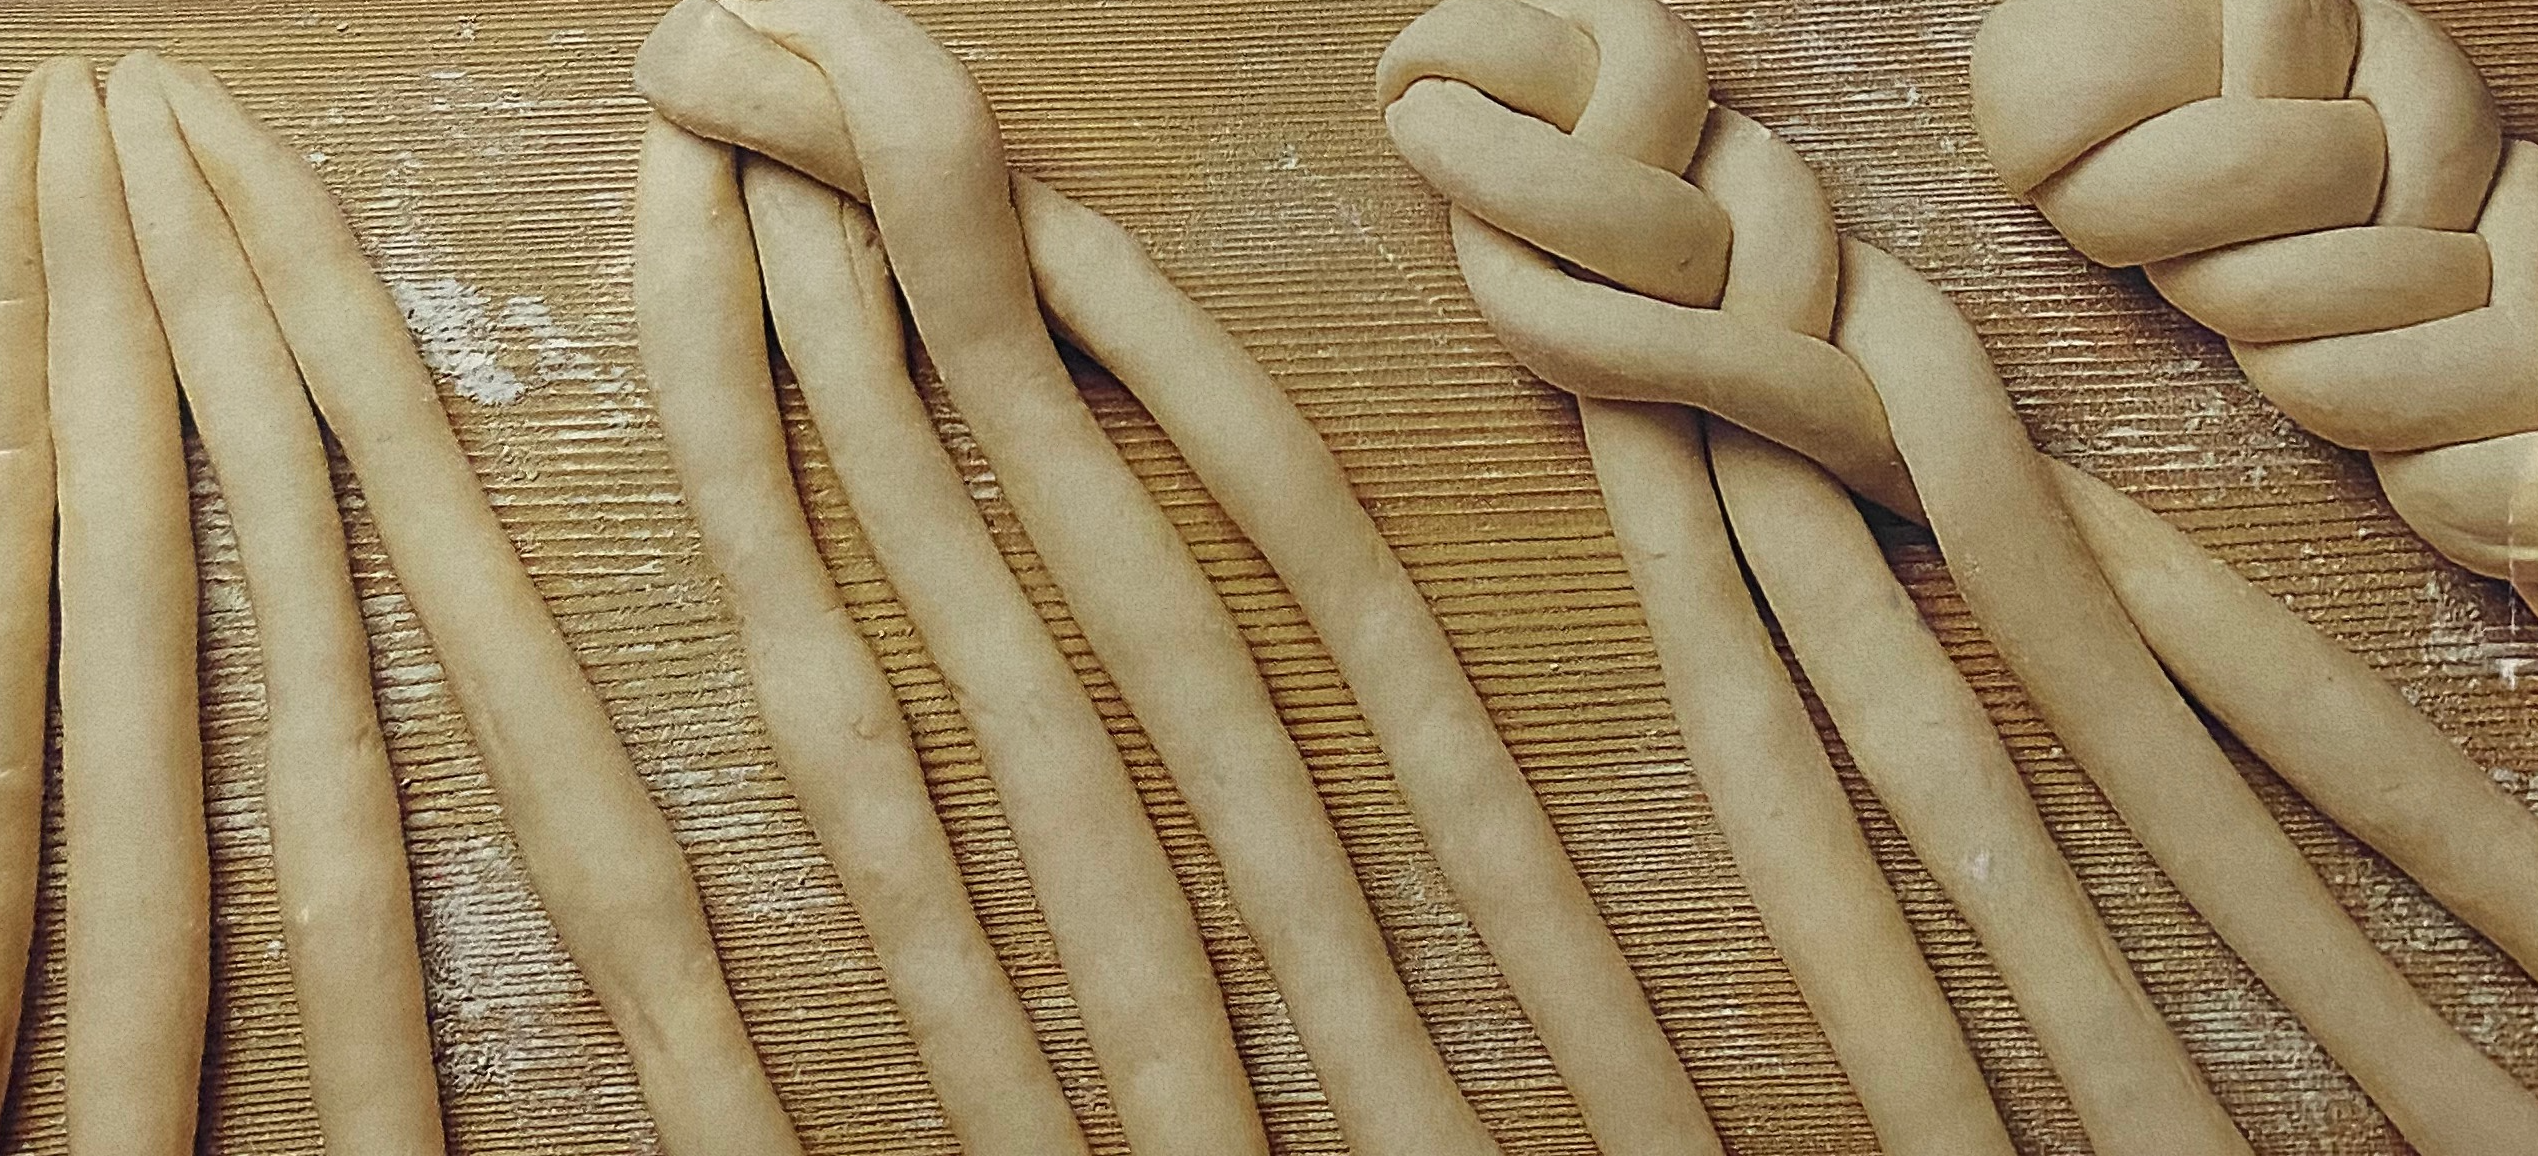
\includegraphics[width=0.48\textwidth]{./assets/tresse_du_dimanche_2}}
        \centerline{\includegraphics[width=0.48\textwidth]{./assets/tresse_du_dimanche_3}}
        \centerline{\includegraphics[width=0.48\textwidth]{./assets/tresse_du_dimanche_4}}
        \columnbreak

        Melangez d'abord la farine, le sel, le sucre et la levure en poudre dans un grand bol.
        \newline

        Ajoutez le lait, le beurre en dés, la levure fraiche dans le même grand bol.
        \newline

        Petrir à la main pendant 10 minutes ou 4 minutes avec la machine en une pate mole est lisse.
        \centerline{\includegraphics[width=0.48\textwidth]{./assets/tresse_du_dimanche}}
        \newline

        Couvrir et laissez doubler de volume pendant minimum 1 heure et demi à temperature ambiante.
        \newline

        Préchauffez le four à 200\textdegree
        \newline

        Coupez la pâte en deux portions, fassonez chacune en un rouleau d'environ 70cm de long aux extrémitées plus fines.
        \newline

        Tressez, déposer sur une plaque chemisé de papier cuisson.
        \newline

        Mélangez le jaune d'oeuf, plus une cuillère de soupe de lait. Dorez la tresse et laissez lever encore envirion 30 minutes.
        \newline

        Dorez encore à l'oeuf et au lait. Cuisson environ 35 à 45 minutes dans la moitié inférieur du four.
        \centerline{\includegraphics[width=0.48\textwidth]{./assets/tresse_du_dimanche_5}}
        \newline
        \newline
        \textbf{Pour 4 personnes}
    \end{multicols}

    \chapter{Repas chaud}
    \newpage

    % Section
    \section{Omelette espagnole}

    \begin{multicols}{2}
        \parbox[1cm]{\textwidth}{
            \begin{description}
                \item
                \textit{3 cuillère à soupe d'huile d'olive}
                \item
                \textit{1 à 2 oignons hachés}
                \item
                \textit{2 gousses d'ail écrasées}
                \item
                \textit{1 poivron rouge évidé et haché}
                \item
                \textit{4 oeufs}
                \item
                \textit{sel et poivre}
                \item
                \textit{2 grosses pommes de terre cuites et émincées}
                \item
                \textit{2 cuillères à soupe de persil haché}
            \end{description}
        }
        \columnbreak

        Faites chauffer 2 cuillères à soupe d'huile dans une poêle de 24 cm, ajoutez et faites revenir les oignons. Ajouter l'ail, le poivron et laissez cuire 10 minutes.
        \newline

        Battez les œufs dans une jatte avec le sel, le poivre, puis ajoutez-leur les pommes de terre, le persil et le mélange précédent.
        \newline

        Faites chauffer le reste d'huile dans la poêle, versez le mélange et laissez cuire 5 minutes, en secouant la poêle.
        \newline
        \newline
        \textbf{Pour 4 personnes}
    \end{multicols}

    \newpage

    % Section
    \section{Curry de haricots}

    \begin{multicols}{2}
        \parbox[1cm]{\textwidth}{
            \begin{description}
                \item
                \textit{500g de haricots noirs ayant trempé une nuit}
                \item
                \textit{sel}
                \item
                \textit{3 cuillères à café de cumin moulu}
                \item
                \textit{1 cuillère à café de garam massala}
                \item
                \textit{1 pincée de Cayenne}
                \item
                \textit{1 cm de gingembre haché}
                \item
                \textit{4 gousses d'ail pilées}
                \item
                \textit{400g de tomates}
                \item
                \textit{3 branches de céleri}
                \item
                \textit{1 cuillère a café de cardamome}
                \item
                \textit{1 cuillère à soupe de coriandre hachée}
                \item
            \end{description}
        }
        \columnbreak

        Égouttez les haricots, mettez-les dans une casserole, couvrez d'eau froide, portez à ébullition et laissez bouillir 10 minutes, puis couvrez et laissez frémir 1h30, en salant à la fin. Mettez de côté 30 cl de liquide de cuisson.
        \newline

        Faites chauffer l'huile dans une casserole, ajoutez et faites revenir les oignons. Ajoutez le cumin, le garam massala, le Cayenne, le gingembre, l'ail et tournez 1 minute. Ajoutez le liquide de cuissons, les haricots, les tomates écrasées, le céleri haché, les grains de cardamome, salez, couvrez et laissez frémir 45 minutes. Ajoutez la coriandre fraîche. Servez avec du riz.
        \newline
        \newline
        \centerline{\includegraphics[width=0.48\textwidth]{./assets/curry_de_haricots}}
        \newline
        \newline
        \textbf{Pour 4 personnes}
        \newline
        \newline
        \centerline{\includegraphics[width=0.48\textwidth]{./assets/curry_de_haricots_fin}}
    \end{multicols}
    \newpage

    % Section
    \section{Risotto milanese}

    \begin{multicols}{2}
        \parbox[1cm]{\textwidth}{
            \begin{description}
                \item
                \textit{1 oignon}
                \item
                \textit{1 gousse d'ail}
                \item
                \textit{1 cuillère à soupe d'huile d'olive}
                \item
                \textit{400g de riz à risotto (ex: arborio)}
                \item
                \textit{1 sachet à safran}
                \item
                \textit{4dl de vin blanc}
                \item
                \textit{1l de bouillon de légume}
                \item
                \textit{50g de parmesan rappé}
                \item
                \textit{sel et poivre}
            \end{description}
        }
        \columnbreak
        \newline
        Pelez l'oignon et l'ail, hachez finement.
        \newline
        Faire chauffer l'huile dans une casserole et y faire revenir l'oignon et l'ail. Ajoutez le riz et le safran, nacrez en remuant. Versez la moitié du vin, faire réduire complètement, ajoutez le reste du vin, faire réduire complètement. Versez peu à peu le bouillon en remuant souvant de manière a juste mouillez le riz à hauteur, laissez mijoter environ 20 minutes jusqu'à ce qu'il soit cremeux et aldante.
        \newline
        Incorporer le parmesan et rectifier l'assaisonnement.
        \newline
        \newline
        \textbf{Pour 4 personnes}
    \end{multicols}
    \newpage

    % Section
    \section{Tarte tata}

    \begin{multicols}{2}
        \parbox[1cm]{\textwidth}{
            \begin{description}
                \item \textit{à faire}
            \end{description}
        }
        \columnbreak
        \newline
        \centerline{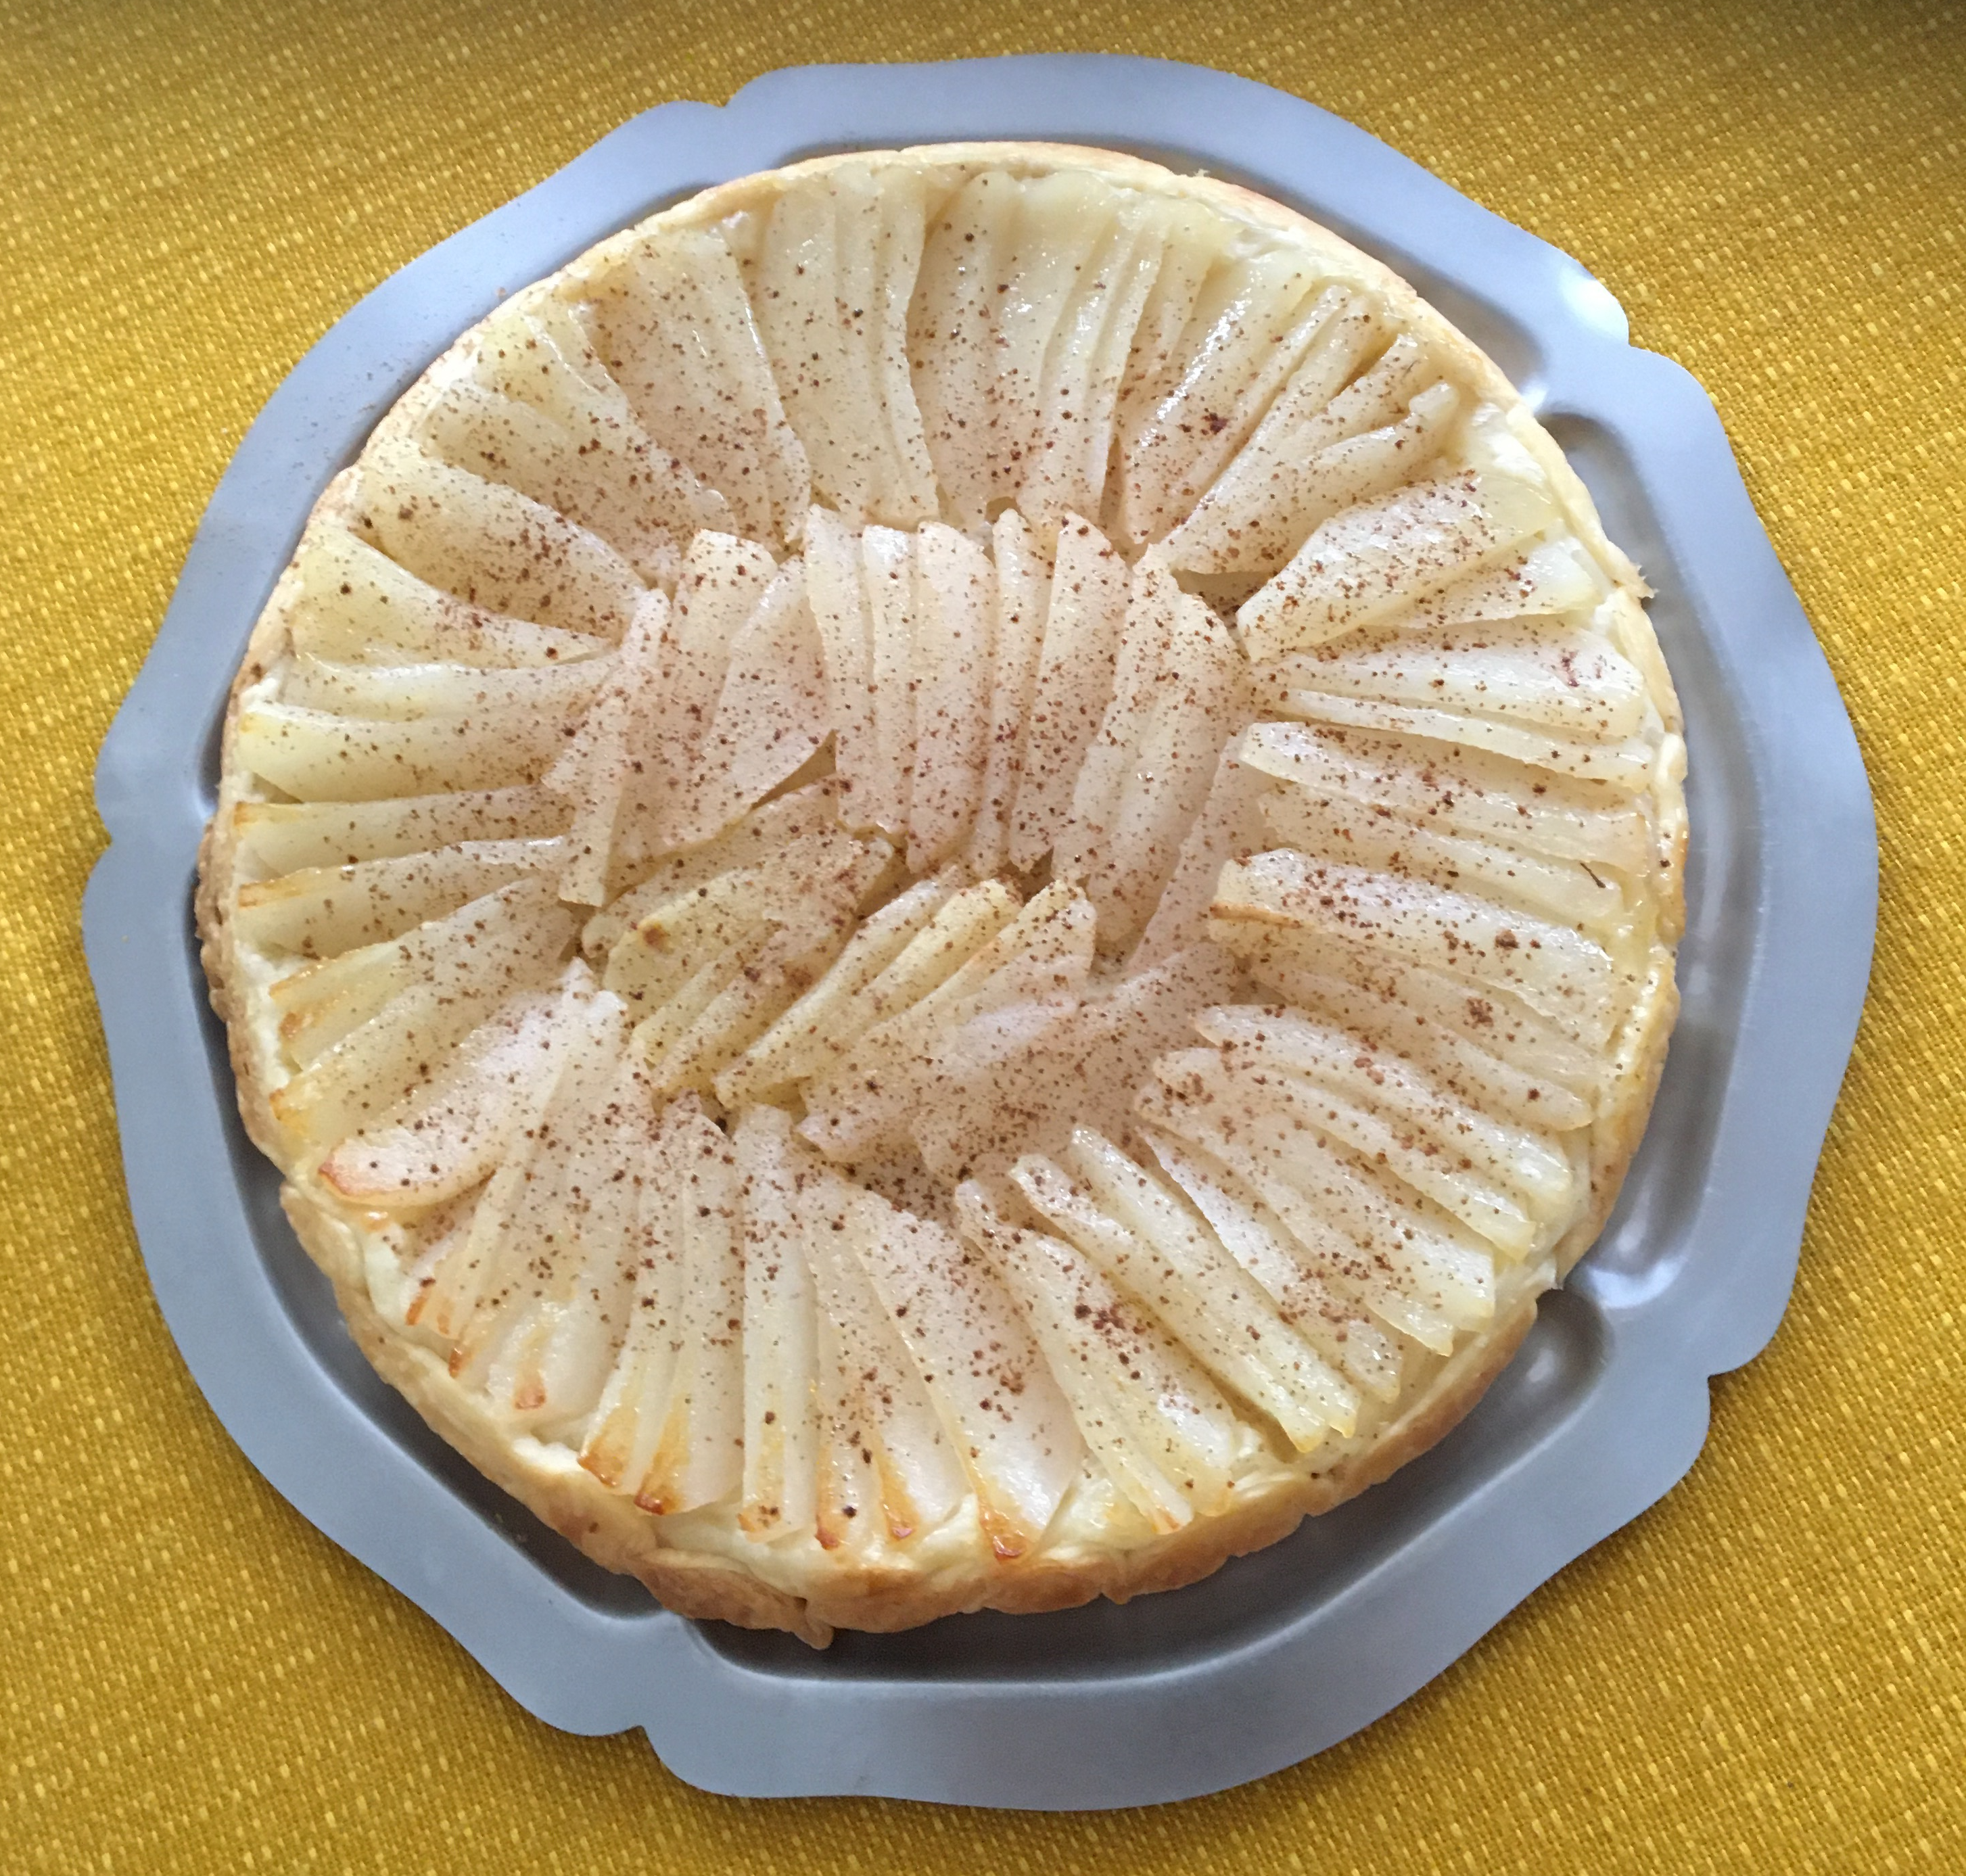
\includegraphics[width=0.48\textwidth]{./assets/tarte_tata}}
        \newline
        \newline
        \textbf{Pour 4 personnes}
    \end{multicols}
    \newpage

    % Section
    \section{Spaghetti végétarien}

    \begin{multicols}{2}
        \parbox[1cm]{\textwidth}{
            \begin{description}
                \item \textit{à faire}
            \end{description}
        }
        \columnbreak

        \textbf{Pour 4 personnes}
    \end{multicols}
    \newpage

    % Section
    \section{Quiche au brocolis}

    \begin{multicols}{2}
        \parbox[1cm]{\textwidth}{
            \begin{description}
                \item
                \textit{PÂTE :}
                \item
                \textit{125g de farine complète}
                \item
                \textit{50g de farine tamisée}
                \item
                \textit{75g de margarine}
                \item
                \textit{50g de gruyère râpé}
                \item
                \textit{1/2 cuillère à café d'herbes de Provence}
                \item
                \textit{1 jaune d'oeuf}
                \item
                \textit{eau glacé}
                \item
                \item {}
                \textit{GARNITURE :}
                \item
                \textit{250g de brocolis}
                \item
                \textit{2 oeufs battus}
                \item
                \textit{15cl de lait}
                \item
                \textit{125g de gruyère râpé}
                \item
                \textit{sel et poivre}
            \end{description}
        }
        \columnbreak
        \newline
        Dans une jatte mélangez les farines avec la margarine. Ajoutez le fromage et les herbes, puis le jaune d'oeuf et de l'eau en quantité suffisante pour obtenir une pâte ferme.
        \newline
        Pêtrissez-la légerement, puis étalez-la et garnissez-en un moule de 20 cm de diamètre. Piquez avec une fourchette et laissez 20 minutes au frais. Couvrez de papier et de haricots, et faire cuire 10 minutes au four (200\textdegree. Reportez à vide au four 5 minutes.)
        \newline
        Pendant ce temps, faites cuire les brocolis à l'eau bouillante salée 5 minutes. Passez-les sous l'eau froide, égouttez-les et coupez-les grossièrement.
        \newline
        Mélangez les oeufs battus avec le lait, les trois quarts du formage, salez, poivrez. Disposez les brocolis sur le fond de tarte, versez dessus ce mélange, saupoudrez du reste de gruyère et remettez au four 35 minutes.
        \newline
        \textbf{Pour 4 personnes}
    \end{multicols}
    \newpage

    % Section
    \section{Tarte aux poireaux}

    \begin{multicols}{2}
        \parbox[1cm]{\textwidth}{
            \begin{description}
                \item \textit{à faire}
            \end{description}
        }
        \columnbreak

        \textbf{Pour 4 personnes}
    \end{multicols}
    \newpage

    \chapter{Desert}
    \newpage

    % Section
    \section{Flon}

    \begin{multicols}{2}
        \parbox[1cm]{\textwidth}{
            \begin{description}
                \item \textit{à faire}
            \end{description}
        }
        \columnbreak

        \textbf{Pour 4 personnes}
    \end{multicols}
    \newpage

\end{document}